\chapter{Sample Final Exam}

\label{sample3}

Here are some worked problems typical for what you might expect on a final examination.

\begin{enumerate}

\item Define the following terms:
\begin{enumerate}
\item An {\it orthogonal matrix}.
\item A {\it basis} for a vector space.
\item The {\it span} of a set of vectors.
\item The {\it dimension} of a vector space.
\item An {\it eigenvector}.
\item A {\it subspace} of a vector space.
\item The {\it kernel} of a linear transformation.
\item The {\it nullity} of a linear transformation.
\item The {\it image} of a linear transformation.
\item The {\it rank} of a linear transformation.
\item The {\it characteristic polynomial} of a square matrix.
\item An {\it equivalence relation}.
\item A {\it homogeneous solution} to a linear system of equations.
\item A {\it particular solution} to a linear system of equations.
\item The {\it general solution} to a linear system of equations.
\item The {\it direct sum} of a pair of subspaces of a vector space.
\item The {\it orthogonal complement} to a subspace of a vector space.
\end{enumerate}




\item {\it Kirchoff's laws}: \index{Kirchoff's laws} Electrical circuits are easy to analyze using systems of equations.
The change in voltage (measured in Volts) around any loop due to batteries $|\big|$
and resistors $/\!\backslash\!/\!\backslash\!/\!\backslash\!/\!\backslash$ (given by the product of the
current measured in Amps and resistance measured in Ohms) equals zero. Also, the sum of currents entering any junction vanishes. Consider the circuit
\[
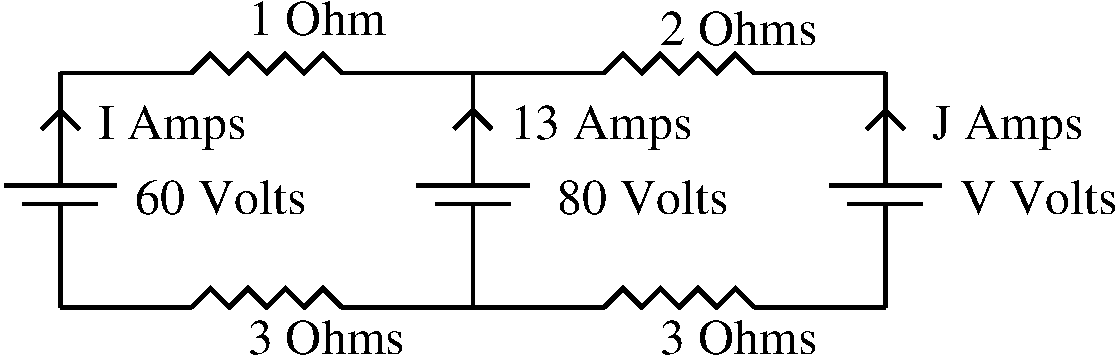
\includegraphics[scale=.6]{circuit.pdf}
\]
Find all possible equations for the unknowns $I$, $J$ and $V$ and then  solve for $I$, $J$ and $V$. Give your answers with correct units.



\item
Suppose $M$ is the matrix of a linear transformation 
\[
L: U\to V
\]
and the vector spaces $U$ and $V$ have dimensions
\[
\mbox{dim}\,  U= n\,,  \qquad \mbox{dim}\,  V= m\, , 
\]
and
\[
m\neq n\, .
\]
Also assume 
\[
\mbox{ker} L = \{0_U\}\, .
\]
\begin{enumerate}
\item How many rows does $M$ have? 
\item How many columns does $M$ have?
\item Are the columns of $M$ linearly independent?
\item What size matrix is $M^TM$?
\item What size matrix is $M M^T$?
\item Is $M^T M$ invertible?
\item is $M^T M$ symmetric? 
\item Is $M^TM$ diagonalizable?
\item  Does $M^TM$ have a zero eigenvalue?
\item Suppose $U=V$ and $\ker L\neq\{0_U\}$. Find an eigenvalue of $M$.
\item  Suppose $U=V$ and $\ker L\neq\{0_U\}$. Find $\det M$.
\end{enumerate}

\item Consider the system of equations
\[
\begin{array}{ccccccccc}
x&+&y&+&z&+&w&=&1\\
x&+&2y&+&2z&+&2w&=&1\\
x&+&2y&+&3z&+&3w&=&1\\
\end{array}
\]
Express this system as a matrix equation $MX=V$ and then find the solution set by computing an $LU$ 
decomposition for the matrix $M$ (be sure to use back and forward substitution).

\item
Compute the following determinants
\begin{gather*}
\det\begin{pmatrix}1&2\\3&4
\end{pmatrix},\:
\det\begin{pmatrix}1&2&3\\4&5&6\\7&8&9
\end{pmatrix},\:
\det\begin{pmatrix}1&2&3&4\\5&6&7&8\\9&10&11&12\\13&14&15&16
\end{pmatrix} ,\:\\
\det\begin{pmatrix}1&2&3&4&5\\6&7&8&9&10\\11&12&13&14&15\\
16&17&18&19&20\\21&22&23&24&25
\end{pmatrix}.
\end{gather*}
Now test your skills on
\[
\det\left(\begin{array}{ccccc}1&2&3&\cdots&n\\n+1&n+2&n+3&\cdots&2n\\2n+1&2n+2&2n+3&&3n \\
\vdots&&&\ddots&\vdots\\n^2-n+1&n^2-n+2&n^2-n+3&\cdots&n^2
\end{array}\right).
\]
{\it Make sure to jot down a few brief notes explaining any clever tricks you use.}

\item
For which values of $a$ does \[U={\rm span} \left\{
\begin{pmatrix}1\\0\\1\end{pmatrix},\begin{pmatrix}1\\2\\-3\end{pmatrix},\begin{pmatrix}a\\1\\0\end{pmatrix}\right\}={\mathbb R}^3\ ?\]
 For any special values of $a$ at which $U\neq{\mathbb R}^3$, express the subspace $U$ as the span of the least number of vectors possible. Give the dimension of $U$ for these cases and
 draw a picture showing $U$ inside ${\mathbb R}^3$.

\item
{\it Vandermonde determinant:}\index{Vandermonde determinant} Calculate the following determinants
\[
\det \begin{pmatrix}1 & x\\ 1 & y\end{pmatrix}\, ,\quad
\det \begin{pmatrix}1 & x & x^2\\ 1 & y&y^2\\ 1& z&z^2\end{pmatrix}\, ,\quad
\det \begin{pmatrix}1 & x & x^2 & x^3\\ 1 & y& y^2 & y^3\\ 1 & z & z^2 & z^3\\ 1 & w & w^2 & w^3\end{pmatrix}\, .
\]
Be sure to factorize you answers, if possible.

{\it Challenging:} Compute the determinant
\[
\det \begin{pmatrix}1 & x_1 & (x_1)^2 & \cdots &(x_1)^{n-1}\\ 
1 & x_2& (x_2)^2 & \cdots &  (x_2)^{n-1}\\ 
1 & x_3& (x_3)^2 & \cdots &  (x_3)^{n-1}\\ 
\vdots &\vdots &\vdots &\ddots & \vdots\ \ \  \\ 
1 & x_n& (x_n)^2 & \cdots &  (x_n)^{n-1}\end{pmatrix}\, .
\]

\item
\begin{enumerate}\item Do the vectors $\left\{\begin{pmatrix}1\\2\\3\end{pmatrix},\begin{pmatrix}3\\2\\1\end{pmatrix},\begin{pmatrix}1\\0\\0\end{pmatrix},\begin{pmatrix}0\\1\\0\end{pmatrix},\begin{pmatrix}0\\0\\1\end{pmatrix}\right\}$ form a basis for ${\mathbb R}^3$? {\it Be sure to justify your answer.}
\item
Find a basis for ${\mathbb R}^4$ that includes the vectors $\begin{pmatrix}1\\2\\3\\4\end{pmatrix}$
and $\begin{pmatrix}4\\3\\2\\1\end{pmatrix}$.
\item Explain in words how to generalize your computation in part (b) to obtain a basis for ${\mathbb R}^n$ that includes a given pair of (linearly independent) vectors $u$ and $v$. 
\end{enumerate}

\item 
Elite NASA engineers\index{Elite NASA engineers} determine that if a satellite is placed in orbit starting at a point ${\cal O}$, it will return
exactly to that same point after one orbit of the earth. Unfortunately, if there is a small mistake in the original location of the 
satellite, which the engineers label by a vector $X$ in ${\mathbb R}^3$ with origin\footnote{This is a spy satellite. The exact location of ${\cal O}$, the orientation of the coordinate axes in ${\mathbb R}^3$ and the unit system employed by the engineers are CIA secrets.} 
at~${\cal O}$, after one orbit the satellite will instead return to some other point $Y\in {\mathbb R}^3$. The engineer's computations
show that $Y$ is related to $X$ by a matrix
\[
Y = \begin{pmatrix} 0&\frac12 & 1 \\[2mm] \frac12 &\frac12 &\frac 12 \\[2mm] 1 & \frac 12 &0\end{pmatrix} X\, .
\]
\begin{enumerate}
\item Find all eigenvalues of the above matrix.
\item Determine  {\it all} possible eigenvectors associated with each eigenvalue.
\end{enumerate}
Let us assume that the rule found by the engineers applies to all subsequent orbits. 
Discuss case by case, what will happen to the satellite if the initial mistake in its location
is in a direction given by an eigenvector. 
\item
In this problem the scalars in the vector spaces are bits ($0,1$ with $1+1=0$). The space $B^k$ is the vector space of bit-valued, $k$-component column vectors.
\begin{enumerate}
\item
Find a basis for $B^3$. 
\item Your answer to part (a) should be a list of vectors $v_1$, $v_2,\ldots v_n$. What number did you find for $n$? 
\item How many elements are there in the {\it set} $B^3$. 
\item What is the dimension of the vector space $B^3$. 
\item Suppose $L:B^3\to B=\{0,1\}$ is a linear transformation. Explain why specifying $L(v_1)$, $L(v_2),\ldots,L(v_n)$ completely determines $L$. 
\item Use the notation of 
part (e) to list {all} linear transformations \[L:B^3\to B\, .\]
How many different linear transformations did you find? Compare your answer to part (c). 
\item Suppose $L_1:B^3\to B$ and $L_2: B^3\to B$ are linear transformations, and $\alpha$ and $\beta$ are bits.
Define a new map 
$(\alpha L_1+\beta L_2):B^3\to B$ by \[(\alpha L_1+\beta L_2)(v)=\alpha L_1(v)+\beta L_2(v).\] Is this map a linear transformation? Explain.
\item Do you think the set of all linear transformations from $B^3$ to $B$ is a vector space using the addition rule above? If you answer yes, 
give a basis for this vector space and state its dimension.
\end{enumerate}

\item
A team of distinguished, post-doctoral engineers analyzes the design for a bridge across the
English channel. They notice that the force on the center of the bridge when it is displaced
by an amount $X=\begin{pmatrix}x\\y\\z\end{pmatrix}$ is given by 
\[
F=\ccolvec{-x-y\\-x-2y-z\\-y-z}\, .
\]
Moreover, having read Newton's Principi\ae\index{Newton's Principi\ae}, they know that force is proportional to acceleration so that\footnote{The bridge is intended for French and English military vehicles, so the exact units, coordinate system and constant of proportionality are state secrets.}
\[
F=\frac{d^2 X}{dt^2}\, .
\]
Since the engineers are worried the bridge might start swaying in the heavy channel winds, they search for 
an oscillatory  solution to this equation of the form\footnote{Here, $a,b,c$ and $\omega$ are constants which we aim to calculate.}
\[
X=\cos(\omega t) \ \begin{pmatrix} a \\ b \\ c\end{pmatrix}\, .
\]
\begin{enumerate}
\item By plugging their proposed solution in the above equations the engineers find an eigenvalue problem
\[
M \begin{pmatrix} a \\ b \\ c\end{pmatrix} = -\omega^2 \begin{pmatrix} a \\ b \\ c\end{pmatrix}\, .
\]
Here $M$ is a $3\times 3$ matrix. Which $3\times 3$ matrix  $M$ did the engineers find?
{\it Justify your answer.}
\item
Find the eigenvalues and eigenvectors of the matrix $M$.
\item The number $|\omega|$ is often called a {\it characteristic frequency}. What characteristic
frequencies do you find for the proposed bridge?
\item Find an orthogonal matrix $P$ such that $MP=PD$ where $D$ is a diagonal matrix.
{\it Be sure to also state your result for $D$.}
\item Is there a direction in which displacing the bridge yields no force? If so give a vector in that direction.
{\it Briefly} evaluate the quality of this bridge design.
\end{enumerate}


\item{\it Conic Sections}:\index{Conic sections} The equation for the most general conic section is given~by
\[
ax^2 + 2bxy+dy^2 + 2cx+2ey + f=0\, . 
\]
Our aim is to analyze the solutions to this equation using matrices.
\begin{enumerate}
\item \label{parta}Rewrite the above quadratic equation as one of the form \[X^T M X +  X^T C + C^T X+ f=0\] relating an unknown column vector $X=\begin{pmatrix}x
 \\ y\end{pmatrix}$, its transpose $X^T$, a $2\times 2$ matrix $M$, a constant column vector $C$ and the  constant~$f$.
\item Does your matrix $M$ obey any special properties? Find its eigenvalues. You may call your answers $\lambda$ and $\mu$ for the rest of the problem to save writing.
\begin{quote}{\it For the rest of this problem we will focus on central conics for which the matrix $M$ is invertible.}\end{quote}
\item Your equation in part (a) above should be be quadratic in $X$. Recall that if $m\neq 0$, 
the quadratic equation $mx^2 + 2cx+f=0$ can be rewritten by {\it completing the square}
\[
m\Big(x+\frac cm\Big)^2 = \frac{c^2}{m}-f\, .
\]
Being very careful that you are now dealing with matrices, use the same trick to rewrite your answer to part (a) in the form
\[
Y^T M Y = g.
\]
Make sure you give formulas for the new unknown column vector~$Y$ and constant $g$ in terms of $X$, $M$, $C$ and $f$. You need not multiply out any of the matrix expressions you find.
\begin{quote}{\it 
If all has gone well, you have found a way to shift coordinates for the original conic equation
to a new coordinate system with its origin at the center of symmetry. Our next aim is to rotate the coordinate
axes to produce a readily recognizable equation.}
\end{quote}
\item Why is the angle between vectors $V$ and $W$ is not changed when you replace
them by $PV$ and $PW$ for $P$ any orthogonal matrix?
\item Explain how to choose an orthogonal  matrix $P$ such that $MP=PD$ where $D$ is a diagonal matrix.
\item For the choice of $P$ above, define our final unknown vector $Z$ by $Y=PZ$. Find an expression for $Y^T MY$ in terms of $Z$ and the eigenvalues of $M$.
\item Call $Z=\begin{pmatrix}z\\w\end{pmatrix}$. What equation do $z$ and $w$ obey?
(Hint, write your answer using $\lambda$, $\mu$ and $g$.)
\item Central conics are circles, ellipses, hyperbolae or a pair of straight lines. Give examples of values of 
$(\lambda,\mu,g)$ which produce each of these cases.

\end{enumerate}

\item Let \(L \colon V \to W\) be a linear transformation between finite-dimensional vector spaces \(V\) and \(W\), and let \(M\) be a matrix for \(L\) (with respect to some basis for \(V\) and some basis for \(W\)). We know that \(L\) has an inverse if and only if it is bijective, and we know a lot of ways to tell whether \(M\) has an inverse. In fact, \(L\) has an inverse if and only if \(M\) has an inverse:
\begin{enumerate}
\item Suppose that \(L\) is bijective (i.e., one-to-one and onto).
\begin{enumerate}
\item Show that \(\dim V=\rank L=\dim W\).
\item Show that \(0\) is not an eigenvalue of \(M\).
\item Show that \(M\) is an invertible matrix. 
\end{enumerate}
\item Now, suppose that \(M\) is an invertible matrix.
\begin{enumerate}
\item Show that \(0\) is not an eigenvalue of \(M\).
\item Show that \(L\) is injective.
\item Show that \(L\) is surjective.
\end{enumerate}
\end{enumerate}

\item Captain Conundrum gives Queen Quandary\index{Queen Quandary} a pair of newborn doves, male and female for her birthday. After one year, this pair of doves breed and produce a pair of dove eggs. One year later these eggs hatch yielding a new pair of doves while the original pair of doves breed again and an additional pair of eggs are laid.  Captain Conundrum is
very happy because now he will never need to buy the Queen a present ever again! 

Let us say that in year zero, the Queen has no doves. In year one she has one pair of doves, in year two she has two pairs of doves {\it etc...}
Call $F_n$ the number of pairs of doves in  years~$n$. For example, $F_0=0$, $F_1=1$ and $F_2=1$. Assume no doves die and that the same breeding pattern continues well into the future. Then $F_3=2$ because the eggs laid by the first pair of doves in year two hatch. Notice also that in year three,  two pairs of eggs are laid (by the first and second pair of doves). Thus $F_4=3$.
\begin{enumerate}
\item Compute $F_5$ and $F_6$.
\item Explain why (for any $n\geq 2$) the following {\it recursion relation}\index{Recursion relation}  holds
\[
F_n=F_{n-1}+F_{n-2}\, .
\]
\item Let us introduce a column vector
$X_n=\begin{pmatrix}\mc{F_n}\\F_{n-1}\end{pmatrix}
$. Compute $X_1$ and~$X_2$. Verify that these vectors obey the relationship
\[
X_2=M X_1 \mbox{ where } M=\begin{pmatrix}1 & 1\\1 & 0\end{pmatrix}\, . \]
\item Show that $X_{n+1}=M X_{n}$.
\item Diagonalize $M$. ({\it I.e.}, write $M$ as a product $M=PDP^{-1}$ where $D$ is diagonal.)
\item Find a simple expression for $M^n$ in terms of $P$, $D$ and $P^{-1}$.
\item Show that $X_{n+1}=M^n X_1$.
\item The number
\[\varphi=\frac{1+\sqrt{5}}2 \]
is called the {\it golden ratio}\index{Golden ratio}. Write the eigenvalues of $M$ in terms of~$\varphi$.
\item Put your results from parts (c), (f) and (g) together (along with a short matrix computation) to find
the formula for the number of doves  $F_n$ in year~$n$ expressed in terms of $\varphi$, $1-\varphi$ and $n$.
\end{enumerate}

\item
Use Gram--Schmidt to find an orthonormal basis for
\[
\mbox{span} 
\left\{
\begin{pmatrix}
1\\1\\1\\1
\end{pmatrix}\, ,\,
\begin{pmatrix}
1\\0\\1\\1
\end{pmatrix}\, ,\,
\begin{pmatrix}
0\\0\\1\\2
\end{pmatrix}
\right\}\, .
\]

\item Let $M$ be the matrix of a linear transformation $L:V\to W$ in given bases for $V$ and $W$.
Fill in the blanks below with one of the following six vector spaces: $V$, $W$, ${\rm ker} L$, 
$\big({\rm ker} L\big)^\perp$, ${\rm im} L$, $\big({\rm im} L\big)^\perp$.
\begin{enumerate}
\item The columns of $M$ span \underline{\phantom{answer}} in the basis given for \underline{\phantom{answer}}.
\item The rows of $M$ span \underline{\phantom{answer}} in the basis given for \underline{\phantom{answer}}.
\end{enumerate} 
Suppose \[M=\begin{pmatrix}1&2&1&3\\2&1&\!-1&2\\1&0&0&\!-1\\4&1&\!-1&0\end{pmatrix}\]
is the matrix of $L$ in the bases $\{v_1,v_2,v_3,v_4\}$ for $V$ and $\{w_1,w_2,w_3,w_4\}$ for~$W$.
Find bases for ${\rm ker} L$ and ${\rm im} L$. Use the dimension formula to check your result.

\item
Captain Conundrum collects the following data set
\[
\begin{array}{c|c}
y&x\\
\hline
5&-2\\
2&-1\\
0&1\\
3&2
\end{array}
\]
which he believes to be well-approximated by a parabola
\[
y=ax^2+bx+c\, .
\]

\begin{enumerate}
\item Write down a system of four linear equations for the unknown coefficients $a$, $b$ and $c$.
\item Write the augmented matrix for this system of equations.
\item Find the reduced row echelon form for this augmented matrix.
\item Are there any solutions to this system?
\item Find the least squares solution to the system.
\item What value does Captain Conundrum predict for $y$ when $x=2$? 
\end{enumerate}


\item Suppose you have collected the following data for an experiment
\[
\begin{array}{l|l}
x&y\\\hline
x_1&y_1\\
x_2&y_2\\
x_3&y_3
\end{array}
\]
and believe that the result is well modeled by a straight line
\[
y=mx+b\, .
\]
\begin{enumerate}
\item Write down a linear system of equations you could use to find the slope $m$ and constant term~$b$. 
\item Arrange the unknowns $(m,b)$ in a column vector $X$ and write your answer to (a) as a matrix equation \[M X= V\, .\]
Be sure to give explicit expressions for the matrix $M$ and column vector $V$.
\item For a generic data set, would you expect your system of equations to have a solution? {\it Briefly} explain your answer.
\item Calculate $M^T M$ and $(M^T M)^{-1}$ (for the latter computation, state the condition required for the inverse to exist).
\item Compute the least squares solution for $m$ and $b$.
\item The least squares method determines a vector $X$ that minimizes the length of the vector $V-MX$. Draw a rough sketch of
the three data points in the $(x,y)$-plane as well as their least squares fit. 
Indicate how the components of $V-MX$ could be obtained from your picture.

\end{enumerate}

\end{enumerate}

\subsection*{Solutions}

\begin{enumerate}
\item You can find the definitions for all these terms by consulting the index of this book.

\item Both junctions give the same equation for the currents
\[
I+J+13=0\, .
\]
There are three voltage loops (one on the left, one on the right and one going around the outside of the circuit). Respectively, they give the equations
\begin{eqnarray}
&60-I-80-3I=0&\nn\\[2mm]
&80+2J-V+3J=0&\nn\\[2mm]
&60-I+2J-V+3J-3I=0&\, .
\end{eqnarray}
The above equations are easily solved (either using an augmented matrix and row reducing, or by substitution). The result is $I=-5$ Amps, $J=-8$ Amps, $V=40$ Volts.



\item 
\begin{enumerate}
\item $m$.
\item $n$.
\item Yes.
\item $n\times n$.
\item $m\times m$.
\item Yes. This relies on ${\rm ker} M=0$ because if $M^T M$ had a non-trivial kernel, then there would be a non-zero solution $X$ to $M^T M X=0$. But then by multiplying on the left by $X^T$ we see that $||MX||=0$. This in turn implies $MX=0$ which contradicts the triviality of the kernel of $M$. 
\item Yes because $\big(M^T M\big)^T=M^T (M^T)^T=M^T M$.
\item Yes, all symmetric matrices have a basis of eigenvectors.
\item No, because otherwise it would not be invertible.
\item Since the kernel of $L$ is non-trivial, $M$ must have $0$ as an eigenvalue.
\item Since $M$ has a zero eigenvalue in this case, its determinant must vanish. {I.e.}, $\det M=0$.
\end{enumerate}

\item To begin with the system becomes
\[
\begin{pmatrix}1&1&1&1\\[1mm]1&2&2&2\\[1mm]1&2&3&3
\end{pmatrix}
\begin{pmatrix}x\\[1mm]y\\[1mm]z\\[1mm]w\end{pmatrix}=
\begin{pmatrix}1\\[1mm]1\\[1mm]1\end{pmatrix}
\]
Then
\begin{gather*}
M=
\begin{pmatrix}
1&1&1&1\\[1mm]1&2&2&2\\[1mm]1&2&3&3
\end{pmatrix}
=
\begin{pmatrix}
1&0&0\\[1mm]1&1&0\\[1mm]1&0&1
\end{pmatrix}
\begin{pmatrix}
1&1&1&1\\[1mm]0&1&1&1\\[1mm]0&1&2&2
\end{pmatrix}\\
=
\begin{pmatrix}
1&0&0\\[1mm]1&1&0\\[1mm]1&1&1
\end{pmatrix}
\begin{pmatrix}
1&1&1&1\\[1mm]0&1&1&1\\[1mm]0&0&1&1
\end{pmatrix}=LU
\end{gather*}
So now $MX=V$ becomes $LW=V$ where $W=UX=\begin{pmatrix}a\\b\\c\end{pmatrix}$ (say). Thus we solve $LW=V$ by forward substitution
\[
a=1,\ a+b=1,  \ a+b+c=1 \Rightarrow a=1,b=0,c=0\, .
\]
Now solve $UX=W$ by back substitution
\begin{gather*}
x+y+z+w=1, \ y+z+w=0, \ z + w =0\\ \ \Rightarrow
w=\mu \mbox{ (arbitrary)}, z=-\mu, y=0, x=1\, .
\end{gather*}
The solution set is $\left\{\begin{pmatrix}x\\y\\z\\y\end{pmatrix}=\begin{pmatrix}1\\0\\-\mu\\\mu\end{pmatrix}: \mu\in {\mathbb R}\right\}$


\item First 
\[\det\begin{pmatrix}1&2\\3&4\end{pmatrix}=-2\, .\]
All the other determinants vanish because the first three rows of each matrix are not independent. 
Indeed, $2R_2-R_1=R_3$ in each case, so we can make row operations to get a row of zeros and thus a zero determinant. 

\item If $U$ spans ${\mathbb R}^3$, then we must be able to express any vector $X=\begin{pmatrix}x\\y\\z\end{pmatrix}$ $\in {\mathbb R}^3$
as
\[
X=c^1\begin{pmatrix}1\\0\\1\end{pmatrix}+c^2\begin{pmatrix}1\\2\\-3\end{pmatrix}+c^3\begin{pmatrix}a\\1\\0\end{pmatrix}
=\begin{pmatrix}1&1&a\\0&2&1\\1&-3&0\end{pmatrix}\begin{pmatrix}c^1\\c^2\\c^3\end{pmatrix}\, ,
\]
for some coefficients $c^1$, $c^2$ and $c^3$. This is a linear system. We could solve for $c^1$, $c^2$ and $c^3$ using an
augmented matrix and row operations. However, since we know that ${\rm dim}\, {\mathbb R}^3=3$, if $U$ spans ${\mathbb R}^3$,
it will also be a basis. Then the solution for  $c^1$, $c^2$ and $c^3$ would be unique. Hence, the $3\times 3$ matrix above must 
be invertible, so we examine its determinant
\[
{\rm det} \begin{pmatrix}1&1&a\\0&2&1\\1&-3&0\end{pmatrix}
=1.(2.0-1.(-3))+1.(1.1-a.2)=4-2a\, .
\]
Thus $U$ spans ${\mathbb R}^3$ whenever $a\neq 2$. When $a=2$ we can write the third vector in $U$ in terms of the preceding ones as
\[
\begin{pmatrix}2\\1\\0\end{pmatrix}=\frac32\begin{pmatrix}1\\0\\1\end{pmatrix}+\frac12\begin{pmatrix}1\\2\\-3\end{pmatrix}.
\]
({\it You can obtain this result, or an equivalent one by studying the above linear system with $X=0$, i.e., the associated homogeneous system.}) The two vectors $\begin{pmatrix}1\\2\\-3\end{pmatrix}$ and $\begin{pmatrix}2\\1\\0\end{pmatrix}$ are clearly linearly independent,
so this is the least number of vectors spanning $U$ for this value of $a$. Also we see that dim$U=2$ in this case. Your picture should be
a plane in ${\mathbb R}^3$ though the origin  containing the vectors $\begin{pmatrix}1\\2\\-3\end{pmatrix}$ and $\begin{pmatrix}2\\1\\0\end{pmatrix}$.

\item 
\begin{gather*}
\det \begin{pmatrix}1 & x\\ 1 & y\end{pmatrix}=y-x\, ,\ \ 
\\
\det \begin{pmatrix}1 & x & x^2\\ 1 & y&y^2\\ 1& z&z^2\end{pmatrix}=
\det \begin{pmatrix}1 & x & x^2\\ 0 & y-x&y^2-x^2\\ 0& z-x&z^2-x^2\end{pmatrix}\\
=(y-x)(z^2-x^2)-(y^2-x^2)(z-x)=(y-x)(z-x)(z-y)\, .
\\
\det \begin{pmatrix}1 & x & x^2 & x^3\\ 1 & y& y^2 & y^3\\ 1 & z & z^2 & z^3\\ 1 & w & w^2 & w^3\end{pmatrix}
=
\det \begin{pmatrix}1 & x & x^2 & x^3\\ 0 & y-x& y^2-x^2 & y^3-x^3\\ 0 & z-x & z^2 -x^2& z^3-x^3\\ 0 & w-x & w^2-x^2 & w^3-x^3\end{pmatrix}
\\
=
\det \begin{pmatrix}1 & 0 & 0 & 0\\ 0 & y-x& y(y-x)& y^2(y-x)\\ 0 & z-x & z(z-x) & z^2(z-x)\\ 0 & w-x & w(w-x) & w^2(w-x)\end{pmatrix}
\\=
(y-x)(z-x)(w-x)\det \begin{pmatrix}1 & 0 & 0 & 0\\ 0 & 1& y& y^2\\ 0 & 1 & z & z^2\\ 0 & 1 & w & w^2\end{pmatrix}
\\
=(y-x)(z-x)(w-x)\det \begin{pmatrix}1 & y & y^2\\ 1 & z&z^2\\ 1& w&w^2\end{pmatrix}
\\
=(y-x)(z-x)(w-x) (z-y)(w-y)(w-z)\, .
\end{gather*}
From the $4\times 4$ case above, you can see all the tricks required for a general Vandermonde matrix.
First zero out the first column by subtracting the first row from all other rows (which leaves the determinant unchanged). Now zero out the top row by subtracting $x_1$ times the first column from the second column,
$x_1$ times the second column from the third column {\it et cetra}. Again these column operations do not
change the determinant. Now factor out $x_2-x_1$ from the second row, $x_3-x_1$ from the third row, {\it etc}. This does change the determinant so we write these factors outside the remaining determinant, which is just the same problem but for the $(n-1)\times(n-1)$ case. Iterating the same procedure gives the result
\[
\det \begin{pmatrix}1 & x_1 & (x_1)^2 & \cdots &(x_1)^{n-1}\\ 
1 & x_2& (x_2)^2 & \cdots &  (x_2)^{n-1}\\ 
1 & x_3& (x_3)^2 & \cdots &  (x_3)^{n-1}\\ 
\mc\vdots &\mc\vdots &\mc\vdots &\ddots & \mc\vdots\ \ \  \\ 
1 & x_n& (x_n)^2 & \cdots &  (x_n)^{n-1}\end{pmatrix}
=\prod_{i>j}(x_i-x_j)\, .
\]
(Here $\prod$ stands for a multiple product, just like $\Sigma$ stands for a multiple sum.)

\item \begin{enumerate}
\item No, a basis for  ${\mathbb R}^3$ must have exactly three vectors.
\item We first extend the original vectors by the standard basis for ${\mathbb R}^4$ and then try to eliminate two of them by considering
\[
\alpha \begin{pmatrix}1\\2\\3\\4\end{pmatrix}+\beta
\begin{pmatrix}4\\3\\2\\1\end{pmatrix} +\gamma 
\begin{pmatrix}1\\0\\0\\0\end{pmatrix}
+\delta\begin{pmatrix}0\\1\\0\\0\end{pmatrix}
+\varepsilon\begin{pmatrix}0\\0\\1\\0\end{pmatrix}
+\eta\begin{pmatrix}0\\0\\0\\1\end{pmatrix}=0\, .
\] 
So we study
\[
\begin{pmatrix}
1&4&1&0&0&0\\
2&3&0&1&0&0\\
3&2&0&0&1&0\\
4&1&0&0&0&1
\end{pmatrix}
\sim
\begin{pmatrix}
1&4&1&0&0&0\\
0&-5&-2&1&0&0\\
0&-10&-3&0&1&0\\
0&-15&-4&0&0&1
\end{pmatrix}
\]
\[
\sim
\begin{pmatrix}
1&0&-\frac35&-4&0&0\\
0&1&\frac25&\frac15&0&0\\[1mm]
0&0&1&10&1&0\\
0&0&2&15&0&1
\end{pmatrix}
\sim
\begin{pmatrix}
1&0&0&2&\frac35&0\\
0&1&0&-\frac{19}5&-\frac25&0\\[1mm]
0&0&1&10&1&0\\
0&0&0&-\frac{5}2&-10&\frac12
\end{pmatrix}
\]
From here we can keep row reducing to achieve RREF, but we can already see that the non-pivot variables will be
$\varepsilon$ and $\eta$. Hence we can eject the last two vectors and obtain as our basis
\[
\left\{
\begin{pmatrix}1\\2\\3\\4\end{pmatrix},
\begin{pmatrix}4\\3\\2\\1\end{pmatrix},
\begin{pmatrix}1\\0\\0\\0\end{pmatrix},
\begin{pmatrix}0\\1\\0\\0\end{pmatrix}
\right\}\, .
\]
Of course, this answer is far from unique!
\item The method is the same as above. Add the standard basis to $\{u,v\}$ to obtain the linearly dependent set
$\{u,v,e_1,\ldots , e_n\}$. Then put these vectors as the columns of a matrix and row reduce. The  standard basis
vectors in columns corresponding to the non-pivot variables can be removed.
\end{enumerate}


\item 
\begin{enumerate}
\item
\[
{\rm det} \begin{pmatrix} \lambda&-\frac12 & -1 \\[2mm] -\frac12 &\lambda-\frac12 &-\frac12 \\[2mm] -1 & -\frac12 &\lambda\end{pmatrix}
=\lambda\Big((\lambda-\frac12\Big)\lambda-\frac14)+\frac12\Big(-\frac{\lambda}2-\frac12\Big)-\Big(-\frac14+\lambda\Big)
\]
\[
=\lambda^3-\frac{1}{2}\lambda^2-\frac32 \lambda=\lambda(\lambda+1)(\lambda-\frac32)\, .
\]
Hence the eigenvalues are $0,-1,\frac32$.
\item
When $\lambda=0$ we must solve the homogenous system
\[
\left(
\begin{array}{ccc|c}
0&\frac12&1&0\\[1mm]
\frac12&\frac12&\frac12&0\\[1mm]
1&\frac12&0&0
\end{array}\right)
\sim
\left(
\begin{array}{ccc|c}
1&\frac12&0&0\\[1mm]
0&\frac14&\frac12&0\\[1mm]
0&\frac12&1&0
\end{array}\right)
\sim
\left(
\begin{array}{ccc|c}
1&0&-1&0\\[1mm]
0&1&2&0\\[1mm]
0&0&0&0
\end{array}\right)\, .
\]
So we find the eigenvector $\begin{pmatrix}s\\-2s\\s\end{pmatrix}$ where $s\neq 0$ is arbitrary.

For $\lambda=-1$ 
\[
\left(
\begin{array}{ccc|c}
1&\frac12&1&0\\[1mm]
\frac12&\frac32&\frac12&0\\[1mm]
1&\frac12&1&0
\end{array}\right)
\sim
\left(
\begin{array}{ccc|c}
1&0&1&0\\[1mm]
0&1&0&0\\[1mm]
0&0&0&0
\end{array}\right)
\, .
\]
So we find the eigenvector $\begin{pmatrix}-s\\0\\s\end{pmatrix}$ where $s\neq 0$ is arbitrary.

Finally, for $\lambda=\frac32$
\[
\left(
\begin{array}{ccc|c}
-\frac32&\frac12&1&0\\[1mm]
\frac12&-1&\frac12&0\\[1mm]
1&\frac12&-\frac32&0
\end{array}\right)
\sim
\left(
\begin{array}{ccc|c}
1&\frac12&-\frac32&0\\[1mm]
0&-\frac54&\frac54&0\\[1mm]
0&\frac54&-\frac54&0
\end{array}\right)
\sim
\left(
\begin{array}{ccc|c}
1&0&-1&0\\[1mm]
0&1&-1&0\\[1mm]
0&0&0&0
\end{array}\right)\, .
\]
So we find the eigenvector $\begin{pmatrix}s\\s\\s\end{pmatrix}$ where $s\neq 0$ is arbitrary.
\end{enumerate}
If the mistake $X$ is in the direction of the eigenvector $\begin{pmatrix}1\\-2\\1\end{pmatrix}$,
then $Y=0$. {\it I.e.}, the satellite returns to the origin ${\cal O}$. For all subsequent orbits it will again return to 
the origin. NASA would be very pleased in this case.

If the mistake $X$ is in the direction $\begin{pmatrix}-1\\0\\1\end{pmatrix}$, then $Y=-X$. Hence the satellite will move to the point opposite to $X$. After next orbit will move back to $X$. It will continue this wobbling
motion indefinitely. Since this is a stable situation, again, the elite engineers will pat themselves on the back.

Finally, if the mistake  $X$ is in the direction $\begin{pmatrix}1\\1\\1\end{pmatrix}$ , the satellite will move
to a point $Y=\frac32 X$ which is further away from the origin. The same will happen for all subsequent
orbits, with the satellite moving a factor $3/2$ further away from ${\cal O}$ each orbit (in reality, after
several orbits, the approximations used by the engineers in their calculations probably fail and a new computation  will be needed). In this case, the satellite will be lost in outer space and the engineers will likely lose their jobs!

\item 
\begin{enumerate}
\item A basis for $B^3$ is $\left\{
\begin{pmatrix}1\\0\\0\end{pmatrix},
\begin{pmatrix}0\\1\\0\end{pmatrix},
\begin{pmatrix}0\\0\\1\end{pmatrix}
\right\}$
\item 3.
\item $2^3=8$.
\item dim$B^3=3$.
\item Because the vectors $\{v_1,v_2,v_3\}$ are a basis any element $v\in B^3$ can be
written uniquely as $v=b^1 v_1 +b^2 v_2+b^3 v_3$ for some triplet of bits~$\begin{pmatrix}b^1\\b^2\\b^3\end{pmatrix}$. Hence, to compute $L(v)$ we use linearity of $L$
\begin{gather*}
L(v) = L(b^1 v_1 +b^2 v_2+b^3 v_3) = b^1 L(v_1)  + b^2 L(v_2) + b^3 L(v_3) \\= \begin{pmatrix}L(v_1) & L(v_2) & L(v_3)\end{pmatrix}
\begin{pmatrix}b^1\\b^2\\b^3\end{pmatrix}\, .
\end{gather*}
\item From the notation of the previous part, we see that we can list  linear transformations $L:B^3\to B$
by writing out all possible bit-valued row vectors
\begin{eqnarray*}
&\begin{pmatrix}0 & 0 & 0\end{pmatrix} ,\\
&\begin{pmatrix}1 & 0 & 0\end{pmatrix} ,\\
&\begin{pmatrix}0 & 1 & 0\end{pmatrix} ,\\
&\begin{pmatrix}0 & 0 & 1\end{pmatrix} ,\\
&\begin{pmatrix}1 & 1 & 0\end{pmatrix} ,\\
&\begin{pmatrix}1 & 0 & 1\end{pmatrix} ,\\
&\begin{pmatrix}0 & 1 & 1\end{pmatrix} ,\\
&\begin{pmatrix}1 & 1  & 1\end{pmatrix} .
\end{eqnarray*}
There are $2^3=8$ different linear transformations $L:B^3\to B$, exactly the same as the number of elements in $B^3$.
\item Yes, essentially just because $L_1$ and $L_2$ are linear transformations. In detail for any bits
$(a,b)$ and vectors $(u,v)$ in $B^3$ it is easy to check the linearity property for $(\alpha L_1+\beta L_2)$
\begin{gather*}(\alpha L_1+\beta L_2)(a u + b v)=\alpha L_1(a u + b v)+\beta L_2(au + bv) 
\\
=\alpha a L_1(u) + \alpha b L_1(v)+ \beta a L_1(u) + \beta b L_1(v) 
\\= a (\alpha L_1(u) + \beta L_2(v))
+ b (\alpha L_1(u) + \beta L_2(v))
\\
=a (\alpha L_1 + \beta L_2)(u) + b  (\alpha L_1 + \beta L_2)(v)\, .
\end{gather*}
Here the first line used the definition of $(\alpha L_1 + \beta L_2)$, the second line depended on
the linearity of $L_1$ and $L_2$, the third line was just algebra and the fourth used the definition of $(\alpha L_1+ \beta L_2)$ again.
\item Yes. The easiest way to see this is the identification above of these maps with bit-valued column vectors. In that notation, a basis is 
\[\Big\{\begin{pmatrix}1&0&0\end{pmatrix},\begin{pmatrix}0&1&0\end{pmatrix},\begin{pmatrix}0&0&1\end{pmatrix}\Big\}\, .\]
Since this (spanning) set has three (linearly independent) elements, the vector space of linear maps $B^3\to B$ has dimension~3. This is an example of a general notion called the {\it dual vector space}\index{Dual vector space}.\end{enumerate}

\item 
\begin{enumerate}
\item $\frac{d^2 X}{dt^2}=\frac{d^2\cos(\omega t )}{dt^2}\colvec{a\\b\\c}=-\omega^2\cos(\omega t) \colvec{a\\b\\c}\, .$ 

Hence
\begin{eqnarray*}
F=\cos(\omega t) \ccolvec{-a-b\\-a-2b-c\\-b-c}&=&\cos(\omega t) \begin{pmatrix}-1&-1&0\\-1&-2&-1\\0&-1&-1\end{pmatrix}\colvec{a\\b\\c}
\\[1mm]&=&-\omega^2\cos(\omega t) \colvec{a\\b\\c}
\, ,\end{eqnarray*}
so 
\[
M=\begin{pmatrix}-1&-1&0\\-1&-2&-1\\0&-1&-1\end{pmatrix}\, .
\]
\item
\begin{eqnarray*}
\det \begin{pmatrix}\lambda+1&\mc1&\mc0\\\mc1&\lambda+2&\mc1\\\mc0&\mc1&\lambda+1\end{pmatrix}
&=&(\lambda+1)\big((\lambda+2)(\lambda+1)-1\big)-(\lambda+1)\\
&=&(\lambda+1)\big((\lambda+2)(\lambda+1)-2\big)\\
&=&(\lambda+1)\big(\lambda^2+3\lambda)=\lambda(\lambda+1)(\lambda+3)\end{eqnarray*}
so the eigenvalues are $\lambda=0,-1 ,-3 $.

For the eigenvectors, when $\lambda=0$ we study:
\[
M-0.I=\begin{pmatrix}-1&-1&0\\-1&-2&-1\\0&-1&-1\end{pmatrix}\sim\begin{pmatrix}1&1&0\\0&-1&-1\\0&-1&-1\end{pmatrix}
\sim\begin{pmatrix}1&0&\!-1\\0&1&1\\0&0&0\end{pmatrix}\, ,
\]
so $\colvec{1\\-1\\1}$ is an eigenvector.

For $\lambda=-1$
\[
M-(-1).I=\begin{pmatrix}0&-1&0\\-1&-1&-1\\0&-1&0\end{pmatrix}\sim\begin{pmatrix}1&0&1\\0&1&0\\0&0&0\end{pmatrix}
\, ,
\]
so $\colvec{-1\\0\\1}$ is an eigenvector.

For $\lambda=-3$
\[
M-(-3).I=\begin{pmatrix}2&-1&0\\-1&1&-1\\0&-1&2\end{pmatrix}\sim\begin{pmatrix}1&-1&1\\0&1&-2\\0&-1&2\end{pmatrix}
\sim\begin{pmatrix}1&0&-1\\0&1&-2\\0&0&0\end{pmatrix}\, ,
\]
so $\colvec{1\\2\\1}$ is an eigenvector.

\item The characteristic frequencies are $0,1,\sqrt{3}$.
\item The orthogonal change of basis matrix 
\[
P=\begin{pmatrix}
\frac1{\sqrt{3}}&-\frac1{\sqrt{2}}&\frac{1}{\sqrt{6}}\\
-\frac1{\sqrt{3}}&\mc 0&\frac{2}{\sqrt{6}}\\
\frac1{\sqrt{3}}&\frac1{\sqrt{2}}&\frac{1}{\sqrt{6}}
\end{pmatrix}
\]
It obeys $MP=PD$ where
\[
D=\begin{pmatrix}0&0&0\\0&-1&0\\0&0&-3\end{pmatrix}\, .
\]
\item Yes, the direction given by the eigenvector $\colvec{1\\-1\\1}$ because its eigenvalue is zero. This is probably a bad design for a bridge because it can be displaced in this direction with no force!
\end{enumerate}

\item 
\begin{enumerate}
\item If we call $M=\begin{pmatrix}a&b\\b&d\end{pmatrix}$, then $X^TMX=ax^2 + 2bxy + dy^2$.
Similarly putting $C=\begin{pmatrix}c\\e\end{pmatrix}$ yields $X^T C + C^T X = 2 X \dotprod C = 2 cx + 2 e y$. Thus
\[
0=
ax^2 + 2bxy + dy^2+2cx+2ey+f\]
\[=\begin{pmatrix} x & y\end{pmatrix} \begin{pmatrix}a&b\\b&d\end{pmatrix}
\begin{pmatrix} x \\ y\end{pmatrix}+ 
\begin{pmatrix} x & y\end{pmatrix}\begin{pmatrix}c\\e\end{pmatrix}+
\begin{pmatrix} c & e\end{pmatrix}\begin{pmatrix}x\\y\end{pmatrix}+f\, .
\]
\item Yes, the matrix $M$ is symmetric, so it will have a basis of eigenvectors and is similar to
a diagonal matrix of real eigenvalues.

To find the eigenvalues notice that $\det\begin{pmatrix}a-\lambda&b\\b&d-\lambda\end{pmatrix}
=(a-\lambda)(d-\lambda)-b^2=\big(\lambda-\frac{a+d}{2}\big)^2-b^2-\big(\frac{a-d}{2}\big)^2$.
So the eigenvalues are \[\lambda=\frac{a+d}{2}+\sqrt{b^2+\big(\frac{a-d}{2}\big)^2}
\mbox{ and } \mu=\frac{a+d}{2}-\sqrt{b^2+\big(\frac{a-d}{2}\big)^2}\, .\]
\item The trick is to write
\[X^T M X + C^T X + X^T C =(X^T+C^T M^{-1}) M (X+M^{-1} C) - C^T M^{-1} C\, ,\]
so that
\[(X^T+C^T M^{-1}) M (X+M^{-1} C) = C^T M C -f\, .\]
Hence $Y=X+M^{-1} C$ and $g=C^T M C -f$.
\item The cosine of the angle between vectors $V$ and $W$ is given by \[\frac{V\dotprod W}{\sqrt{V\dotprod V\, W\dotprod W}}=\frac{V^T W}{\sqrt{V^T V\, W^T W}}\, .\] 
So replacing $V\to PV$ and $W\to PW$ will always give a factor $P^T P$ inside all the products, but $P^TP=I$ for orthogonal matrices. Hence none of the dot products in the above formula changes, so 
neither does the angle between $V$ and $W$.
\item If we take the eigenvectors of $M$, normalize them ({\it i.e.} divide them by their lengths),
and put them in a matrix $P$ (as columns) then $P$ will be an orthogonal matrix. (If it happens
that $\lambda=\mu$, then we also need to make sure the eigenvectors spanning the two dimensional
eigenspace corresponding to $\lambda$ are orthogonal.) Then, since $M$ times the eigenvectors
yields just the eigenvectors back again multiplied by their eigenvalues, it follows that $MP=PD$
where $D$ is the diagonal matrix made from eigenvalues.
\item If $Y=PZ$, then $Y^T M Y= Z^T P^T M P Z = Z^T P^T P D Z = Z^T D Z$ where $D=\begin{pmatrix}\lambda & 0 \\ 0&\mu \end{pmatrix}$.
\item Using part (f) and (c) we have 
\[\lambda z^2 + \mu w^2 = g\, .\]
\item When $\lambda=\mu$ and $g/\lambda=R^2$, we get the equation for a circle radius $R$ in the $(z,w)$-plane. When $\lambda$, $\mu$ and $g$ are postive, we have the equation for an ellipse. Vanishing $g$ along with $\lambda$ and $\mu$ of opposite signs gives a pair of straight lines.
When $g$ is non-vanishing, but $\lambda$ and $\mu$ have opposite signs, the result is a pair of hyperbol\ae. These shapes all come from cutting a cone with a plane, and are therefore called
conic sections.
\end{enumerate}

\item  We  show  that  \(L\)  is  bijective  if  and  only  if  \(M\)  is  invertible.
 		\begin{enumerate}
 		\item  We  suppose  that  \(L\)  is  bijective.
 		\begin{enumerate}
 		\item  Since  \(L\)  is  injective,  its  kernel  consists  of  the  zero  vector  alone.  Hence
 		\[
 		\null  L=\dim  \ker  L=0.
 		\]
 		So  by  the  Dimension  Formula,
 		\[
 		\dim  V=\null  L+\rank  L=\rank  L.
 		\]
 		Since  \(L\)  is  surjective,  \(L(V)=W.\)  Thus
 		\[
 		\rank  L=\dim  L(V)=\dim  W.
 		\]
 		Thereby  \[\dim  V=\rank  L=\dim  W.\]
 		\item  Since  \(\dim  V=\dim  W\),  the  matrix  \(M\)  is  square  so  we  can  talk  about  its  eigenvalues.  Since  \(L\)  is  injective,  its  kernel  is  the  zero  vector  alone.  That  is,  the  only  solution  to  \(LX=0\)  is  \(X=0_V\).  But  \(LX\)  is  the  same  as  \(MX\),  so  the  only  solution  to  \(MX=0\)  is  \(X=0_V\).  So  \(M\)  does  not  have  zero  as  an  eigenvalue.
 		\item  Since  \(MX=0\)  has  no  non-zero  solutions,  the  matrix  \(M\)  is  invertible.
	\end{enumerate}
 		\item  Now  we  suppose  that  \(M\)  is  an  invertible  matrix.
 		\begin{enumerate}
 		\item  Since  \(M\)  is  invertible,  the  system  \(MX=0\)  has  no  non-zero  solutions.  But  \(LX\)  is  the  same  as  \(MX\),  so  the  only  solution  to  \(LX=0\)  is  \(X=0_V\).  So  \(L\)  does  not  have  zero  as  an  eigenvalue.
 		\item  Since  \(LX=0\)  has  no  non-zero  solutions,  the  kernel  of  \(L\)  is  the  zero  vector  alone.  So  \(L\)  is  injective.
 		\item  Since  \(M\)  is  invertible,  we  must  have  that  \(\dim  V=\dim  W\).  By  the  Dimension  Formula,  we  have
 		\[
 		\dim  V=\null  L+\rank  L
 		\]
 		and  since  \(\ker  L=\{0_V\}\)  we  have  \(\null  L=\dim  \ker  L=0\),  so
 		\[
 		\dim  W=\dim  V=\rank  L=\dim  L(V).
 		\]
 		Since  \(L(V)\)  is  a  subspace  of  \(W\)  with  the  same  dimension  as  \(W\),  it  must  be  equal  to  \(W\).  To  see  why,  pick  a  basis  \(B\)  of  \(L(V)\).  Each  element  of  \(B\)  is  a  vector  in  \(W\),  so  the  elements  of  \(B\)  form  a  linearly  independent  set  in  \(W\).  Therefore  \(B\)  is  a  basis  of  \(W\),  since  the  size  of  \(B\)  is  equal  to  \(\dim  W\).  So  \(L(V)=\spa  B=W.\)  So  \(L\)  is  surjective.
 		\end{enumerate}
 		\end{enumerate}

\item 
\begin{enumerate}
\item $F_4=F_2+F_3=2+3=5$.
\item The number of pairs of doves in any given year equals the number of the previous years plus those that hatch and there are as many of them as pairs of doves in the year before the previous year.
\item $X_1=\begin{pmatrix}F_1\\F_0\end{pmatrix}=\begin{pmatrix}1\\0\end{pmatrix}$
and $X_2=\begin{pmatrix}F_2\\F_1\end{pmatrix}=\begin{pmatrix}1\\1\end{pmatrix}$.
\[
MX_1=\begin{pmatrix}1 & 1\\ 1& 0\end{pmatrix}\begin{pmatrix}1\\ 0\end{pmatrix}
=\begin{pmatrix}1\\1\end{pmatrix}=X_2\, .
\]
\item We just need to use the recursion relationship of part (b) in the top slot of $X_{n+1}$:
\[
X_{n+1}=\ccolvec{F_{n+1}\\F_n}
=\ccolvec{F_{n}+F_{n-1}\\F_n}=
\begin{pmatrix}1 & 1\\ 1& 0\end{pmatrix}\ccolvec{F_{n}\\F_{n-1}}=M X_n\, .
\]
\item Notice $M$ is symmetric so this is guaranteed to work. \[\det \begin{pmatrix}1-\lambda&\mc1\\\mc1&-\lambda\end{pmatrix}=\lambda(\lambda-1)-1=\big(\lambda-\frac12\big)^2-\frac54\, ,\]
so the eigenvalues are $\frac{1\pm\sqrt{5}}{2}$. Hence the eigenvectors are $\ccolvec{\frac{1\pm\sqrt{5}}{2}\\1}$, respectively (notice that $\frac{1+\sqrt{5}}{2}+1=\frac{1+\sqrt{5}}{2}.\frac{1+\sqrt{5}}{2}$ and $\frac{1-\sqrt{5}}{2}+1=\frac{1-\sqrt{5}}{2}.\frac{1-\sqrt{5}}{2}$).
Thus $M=PDP^{-1}$ with \[D=\begin{pmatrix}\frac{1+\sqrt{5}}{2}&\mc0\\[1mm]\mc0&\frac{1-\sqrt{5}}{2}\end{pmatrix} \mbox{ and } P =\begin{pmatrix}\frac{1+\sqrt{5}}{2}&\frac{1-\sqrt{5}}{2}\\[1mm]\mc1&\mc1\end{pmatrix}\, .\]
\item $M^n=(P D P^{-1})^n = P D P^{-1} P D P^{-1} \ldots P D P^{-1} = P D^n P^{-1}$.
\item Just use the matrix recursion relation of part (d) repeatedly: \[X_{n+1}= M X_{n} = M^2 X_{n-1}=\cdots = M^{n} X_1\, .\]
\item The eigenvalues are $\varphi = \frac{1+\sqrt{5}}{2}$ and $1-\varphi = \frac{1-\sqrt{5}}{2}$.
\item \begin{gather*}X_{n+1}=\ccolvec{F_{n+1}\\F_n}=
M^n X_n = P D^n P^{-1} X_{1}\\=P 
\begin{pmatrix}\varphi&\mc0\\\mc0&1-\varphi\end{pmatrix}^{\!n} 
\begin{pmatrix}\frac{1}{\sqrt{5}}&\star \\-\frac{1}{\sqrt{5}}& \star\end{pmatrix}
\begin{pmatrix}1\\ 0\end{pmatrix}
=P 
\begin{pmatrix}\varphi^n&\mc0\\\mc0&(1-\varphi)^n\end{pmatrix}
\begin{pmatrix}\frac{1}{\sqrt{5}}\\-\frac{1}{\sqrt{5}}\end{pmatrix}
\\
=\begin{pmatrix}\frac{1+\sqrt{5}}{2}&\frac{1-\sqrt{5}}{2}\\[1mm]\mc1&\mc1\end{pmatrix}
\begin{pmatrix}\mc{\frac{\varphi^n}{\sqrt{5}}}\\[1mm]-\frac{(1-\varphi)^n}{\sqrt{5}}\end{pmatrix}
=\begin{pmatrix}\mc\star \\[1mm]\frac{\varphi^n-(1-\varphi)^n}{\sqrt{5}}\end{pmatrix}.
\end{gather*}
Hence
\[F_n=\frac{\varphi^n-(1-\varphi)^n}{\sqrt{5}}\, .\]
These are the famous Fibonacci numbers\index{Fibonacci numbers}.
\end{enumerate}


\item Call the three vectors $u,v$ and $w$, respectively. Then
\[
v^\perp=v-\frac{u\dotprod v}{u\dotprod u} u =v-\frac34 u = \begin{pmatrix}\frac14 \\[1mm] -\frac34 \\[1mm] \frac14\\[1mm] \frac14\end{pmatrix}\, ,
\]
and
\[
w^\perp = w - \frac{u\dotprod w}{u\dotprod u} u-\frac{v^\perp\dotprod w}{v^\perp\dotprod v^\perp} v^\perp
=w-\frac{3}{4} u -\frac{\frac34}{\frac34}v^\perp =\begin{pmatrix}-1\\0\\0\\1\end{pmatrix}
\]
Dividing by lengths, an orthonormal basis for ${\rm span}\{u,v,w\}$ is
\[
\left\{\begin{pmatrix}\frac12\\[2mm]\frac12\\[2mm]\frac12\\[2mm]\frac12\end{pmatrix},
\begin{pmatrix}\frac{\sqrt{3}}6\\[1mm]-\frac{\sqrt{3}}2\\[1mm]\frac{\sqrt{3}}6\\[1mm]\frac{\sqrt{3}}6\end{pmatrix},
\begin{pmatrix}-\frac{\sqrt{2}}2\\[1mm]\mc0\\[1mm]\mc0\\[1mm]\frac{\sqrt{2}}2\end{pmatrix}
\right\}\, .
\]
\item 

\begin{enumerate}
\item The columns of $M$ span ${\rm im} L$ in the basis given for $W$.
\item The rows of $M$ span $({\rm ker}L)^\perp$% in the basis given for $V$.
\item First we put $M$ in RREF:
\begin{eqnarray*}
M& = & \begin{pmatrix}1&2&1&3\\2&1&\!-1&2\\1&0&0&\!-1\\4&1&\!-1&0\end{pmatrix}
\ \sim\
\begin{pmatrix}1&2&1&3\\0&-3&-3&-4\\0&-2&-1&-4\\0&-7&-5&\!-12\end{pmatrix}\\[2mm]
&\sim& 
\begin{pmatrix}1&0&-1&\frac13\\[1mm]0&1&1&\frac43\\[1mm]0&0&1&-\frac43\\[1mm]0&0&2&-\frac83\end{pmatrix}
\ \sim\ \begin{pmatrix}1&0&0&-1\\[1mm]0&1&0&\frac83\\[1mm]0&0&1&-\frac43\\[1mm]0&0&0&0\end{pmatrix}\, .
\end{eqnarray*}
Hence \[\ker L=\spa\{v_1-\frac83v_2+\frac43 v_3+v_4\}\] and \[{\rm im} L=\spa\{v_1+2v_2+v_3+4v_4,2v_1+v_2+v_4,v_1-v_2-v_4\}\, .\]
Thus $\dim\ker L=1$ and $\dim{\rm im} L=3$ so \[\dim\ker L+\dim{\rm im} L=1+3=4=\dim V\, .\]
\end{enumerate}

\item 
\begin{enumerate}
\item
\[
\left\{
\begin{array}{l}
5=4a-2b+c\\
2=a-b+c\\
0=a+b+c\\
3=4a+2b+c\, .
\end{array}
\right.
\]
\item[(b,c,d)]
\[
\left(
\begin{array}{rrr|r}
4&-2&1&5\\
1&-1&1&2\\
1&1&1&0\\
4&2&1&3
\end{array}
\right)
\sim
\left(
\begin{array}{rrr|r}
1&1&1&0\\
0&-6&-3&5\\
0&-2&0&2\\
0&-2&-3&3
\end{array}
\right)
\sim
\left(
\begin{array}{rrr|r}
1&0&1&-1\\
0&1&0&1\\
0&0&-3&11\\
0&0&-3&3
\end{array}
\right)
\]
The system has no solutions because $c=-1$ and $c=-\frac{11}{3}$ is impossible.
\item[(e)]
Let \[M=\begin{pmatrix}
4&-2&1\\
1&-1&1\\
1&1&1\\
4&2&1
\end{pmatrix}\mbox{ and }
V=\colvec{5\\2\\0\\3}\, .\]
Then 
\[
M^T M=\begin{pmatrix}34&0&10\\0&10&0\\10&0&4\end{pmatrix}
\mbox{ and } 
M^TV=\colvec{34\\-6\\10}\, .
\]
So 
\[
\begin{amatrix}{3}
 34&0&10&34\\0&10&0&-6\\10&0&4&10
\end{amatrix}
~\sim
\begin{amatrix}{3}
1&0&\frac25&1\\0&10&0&-6\\0&0&-\frac{18}5&0
\end{amatrix}
~\sim
\begin{amatrix}{3}
1&0&0&1\\0&1&0&-\frac35\\0&0&1&0
\end{amatrix}
\]
The least squares solution is $a=1$, $b=-\frac35$ and $c=0$.
\item The Captain predicts $y(2)=1.2^2-\frac35.2+0=\frac{14}5$.
\end{enumerate}
 
\item 
%\item We show that \(L\) is bijective if and only if \(M\) is invertible.
%\begin{enumerate}
%\item We suppose that \(L\) is bijective.
%\begin{enumerate}
%\item Since \(L\) is injective, its kernel consists of the zero vector alone. So
%\[
%\null L=\dim \ker L=0.
%\]
%By the dimension formula,
%\[
%\dim V=\null L+\rank L=\rank L.
%\]
%Since \(L\) is surjective, \(L(V)=W.\) So
%\[
%\rank L=\dim L(V)=\dim W.
%\]
%So \[\dim V=\rank L=\dim W.\]
%\item Since \(\dim V=\dim W\), the matrix \(M\) is square so we can talk about its eigenvalues. Since \(L\) is injective, its kernel is the zero vector alone. That is, the only solution to \(LX=0\) is \(X=0_V\). But \(LX\) is the same as \(MX\), so the only solution to \(MX=0\) is \(X=0_V\). So \(M\) does not have zero as an eigenvalue.
%\item Since \(MX=0\) has no non-zero solutions, the matrix \(M\) is invertible.
%\end{enumerate}
%\item Now we suppose that \(M\) is an invertible matrix.
%\begin{enumerate}
%\item Since \(M\) is invertible, the system \(MX=0\) has no non-zero solutions. But \(LX\) is the same as \(MX\), so the only solution to \(LX=0\) is \(X=0_V\). So \(L\) does not have zero as an eigenvalue.
%\item Since \(LX=0\) has no non-zero solutions, the kernel of \(L\) is the zero vector alone. So \(L\) is injective.
%\item Since \(M\) is invertible, we must have that \(\dim V=\dim W\). By the Dimension Formula, we have
%\[
%\dim V=\null L+\rank L
%\]
%and since \(\ker L=\{0_V\}\) we have \(\null L=\dim \ker L=0\), so
%\[
%\dim W=\dim V=\rank L=\dim L(V).
%\]
%Since \(L(V)\) is a subspace of \(W\) with the same dimension as \(W\), it must be equal to \(W\). To see why, pick a basis \(B\) of \(L(V)\). Each element of \(B\) is a vector in \(W\), so the elements of \(B\) form a linearly independent set in \(W\). Therefore \(B\) is a basis of \(W\), since the size of \(B\) is equal to \(\dim W\). So \(L(V)=\spa B=W.\) So \(L\) is surjective.
%\end{enumerate}
%\end{enumerate}





\end{enumerate}

\newpage
